\subsection{Китай}
\textit{Здание Министерства финансов (наб. Мойки, 45)}




Китай был крайне ослабшим государством в конце XIX - начале XX века, чем пользовались все мировые державы на протяжении XIX века. Например, Российская империя вела экспансию на Дальнем востоке за счет территорий Китая, но она так не смогла заполучить выход к незамерзающему порту.

Поэтому Россию активно заинтересовала территория Маньчжурии,

\textit{Вставка изображения}


{\centering 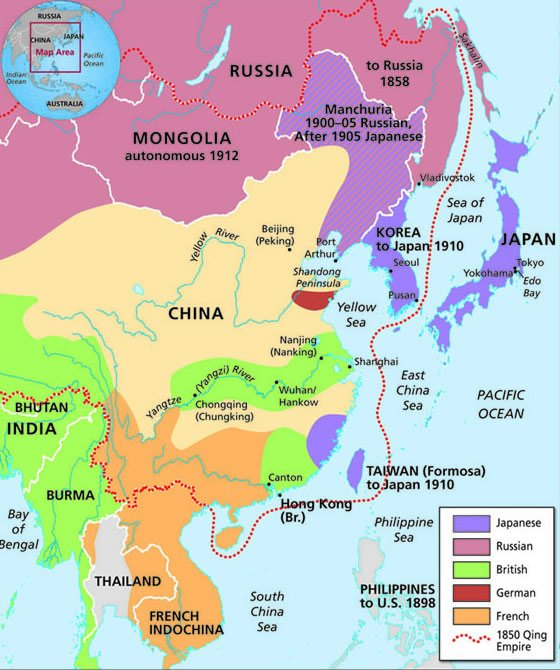
\includegraphics[width=0.7\textwidth]{images/Spheres-Influence-Chinese.jpeg}}  

вместе с Ляодунским полуостровом, где можно было, наконец, получить незамерзающий порт. 
К началу XX века серьезную силу набрала Япония, а вместе с ними и амбиции. Токио хотел заполучить территории Кореи, которые были подконтрольны Китаю, из-за территориальной близости региона, а также из-за ресурсов, расположенных на полуострове. В 1895-1896 проходила Японско-Китайская война, где Китай был разгромлен, а Япония получила желаемые территории, а также Порт-Артур. Тут уже вмешались Европейские державы, включая Россию, и заставили Японию отказаться от Порт-Артура. Здесь сыграла Российская дипломатия, и территория порта была взята в Аренду Российской Империей.

\textit{Возвращаемся к живому кадру со мной на набережной Мойки}

После Японско-Китайской войны стало ясно: Китай не сможет защитить себя от Японской агрессии, из-за чего он начал искать защиту на стороне. Был заключен Ли-Лобановский договор (1966) между Российской империей и Китаем. Россия обязывалась выступать в роли защитника, а взамен требовала иметь возможность построить свои ветки железнодорожных путей на территории Маньчжурии, что укорачивало транс-сибирскую магистраль, выставить свои войска для обороны ЖД путей, создается Русско-Китайский банк, который спонсировал строительство и позволял влиять на экономику региона, а также усиливало политическую зависимость Китая от России. 

С 1898 по 1901 в Китае бушевало боксерское восстание, которое было направлено против иностранных администраций в Китае. Китай не хотел подавлять эти восстания и Европейские державы самостоятельно ввели войска в регион,

\textit{Вставка видеохроник с кадрами Китая, кораблей Европейских держав, и Европейскими/Японскими военными на улицах Китая}

что ещё сильнее ослабило Китай. После подавления восстания основные войска других стран были выведены, но Российская империя оставила свои гарнизоны в Маньчжурии, взяв регион под свой контроль без официальной экспансии. Всё это крайне не нравилось Британской империи: мало того, что Россия закреплялась на незамерзающем порту, чему Британия препятствовала длительное время, так к тому же Лондон выступал за политику "открытых дверей" в Китае, что подразумевало свободную торговлю, а Россия своими движениями в регионе разделяла большой рынок Китая на сферы влияния, что препятствовало продаже Британских товаров. На этой почве Британия нашла выгодным решением помочь Японии в борьбе с Россией в регионе.